\chapter{Appendix}

Kan forklare hvis jeg går til sidespor, skal tage censor i hånden,

Appendix er til ting man ikke mener er nødvendige til hovedrapporten, men stadig er relevante for censor at vide

\begin{figure}[htbp]
     \centering
     % Første Billede (Øverst)
     \begin{subfigure}[b]{\textwidth}
         \centering
         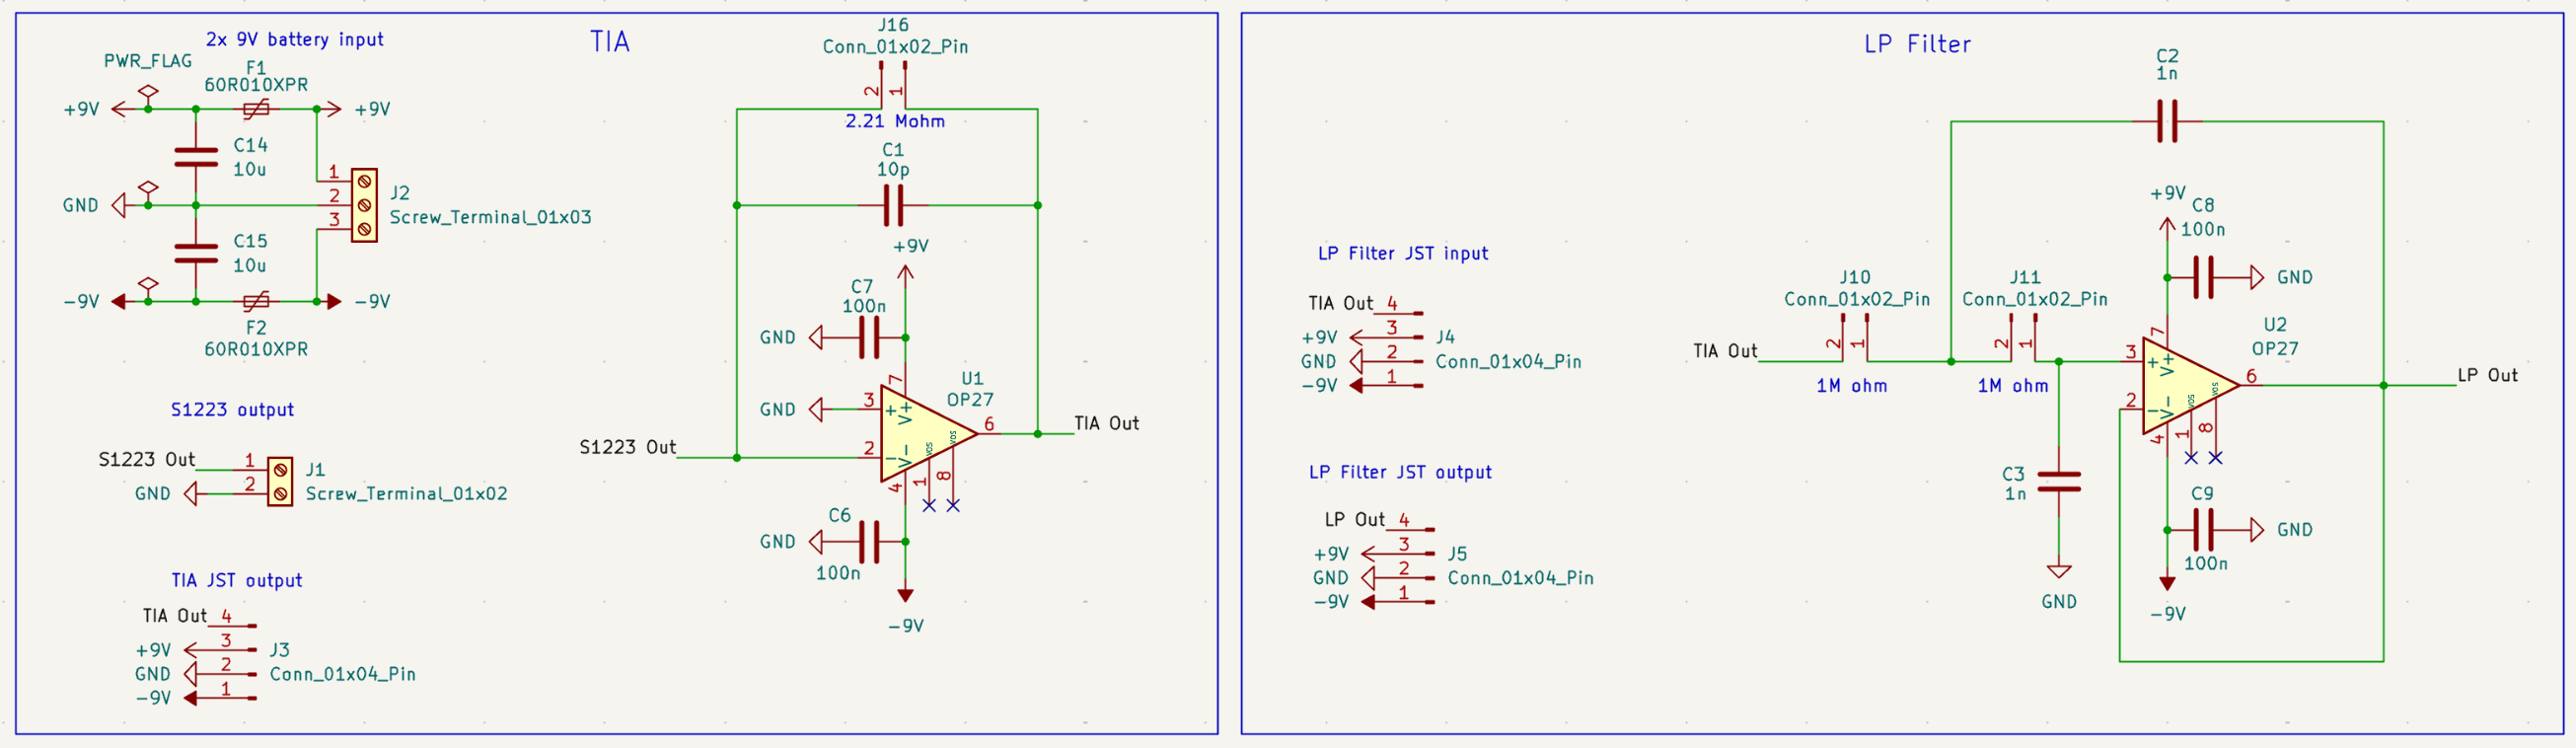
\includegraphics[width=0.8\textwidth]{Pictures/PCB/TIA_LOWPASS.png}
         \caption{Skematisk diagram af Trans Impedance Amplifier(TIA) og lavpasfilter.}
         \label{fig:TIA_LP}
     \end{subfigure}
     
     \vspace{1cm} % Tilføjer vertikal afstand mellem de to billeder

     % Andet Billede (Nederst)
     \begin{subfigure}[b]{\textwidth}
         \centering
         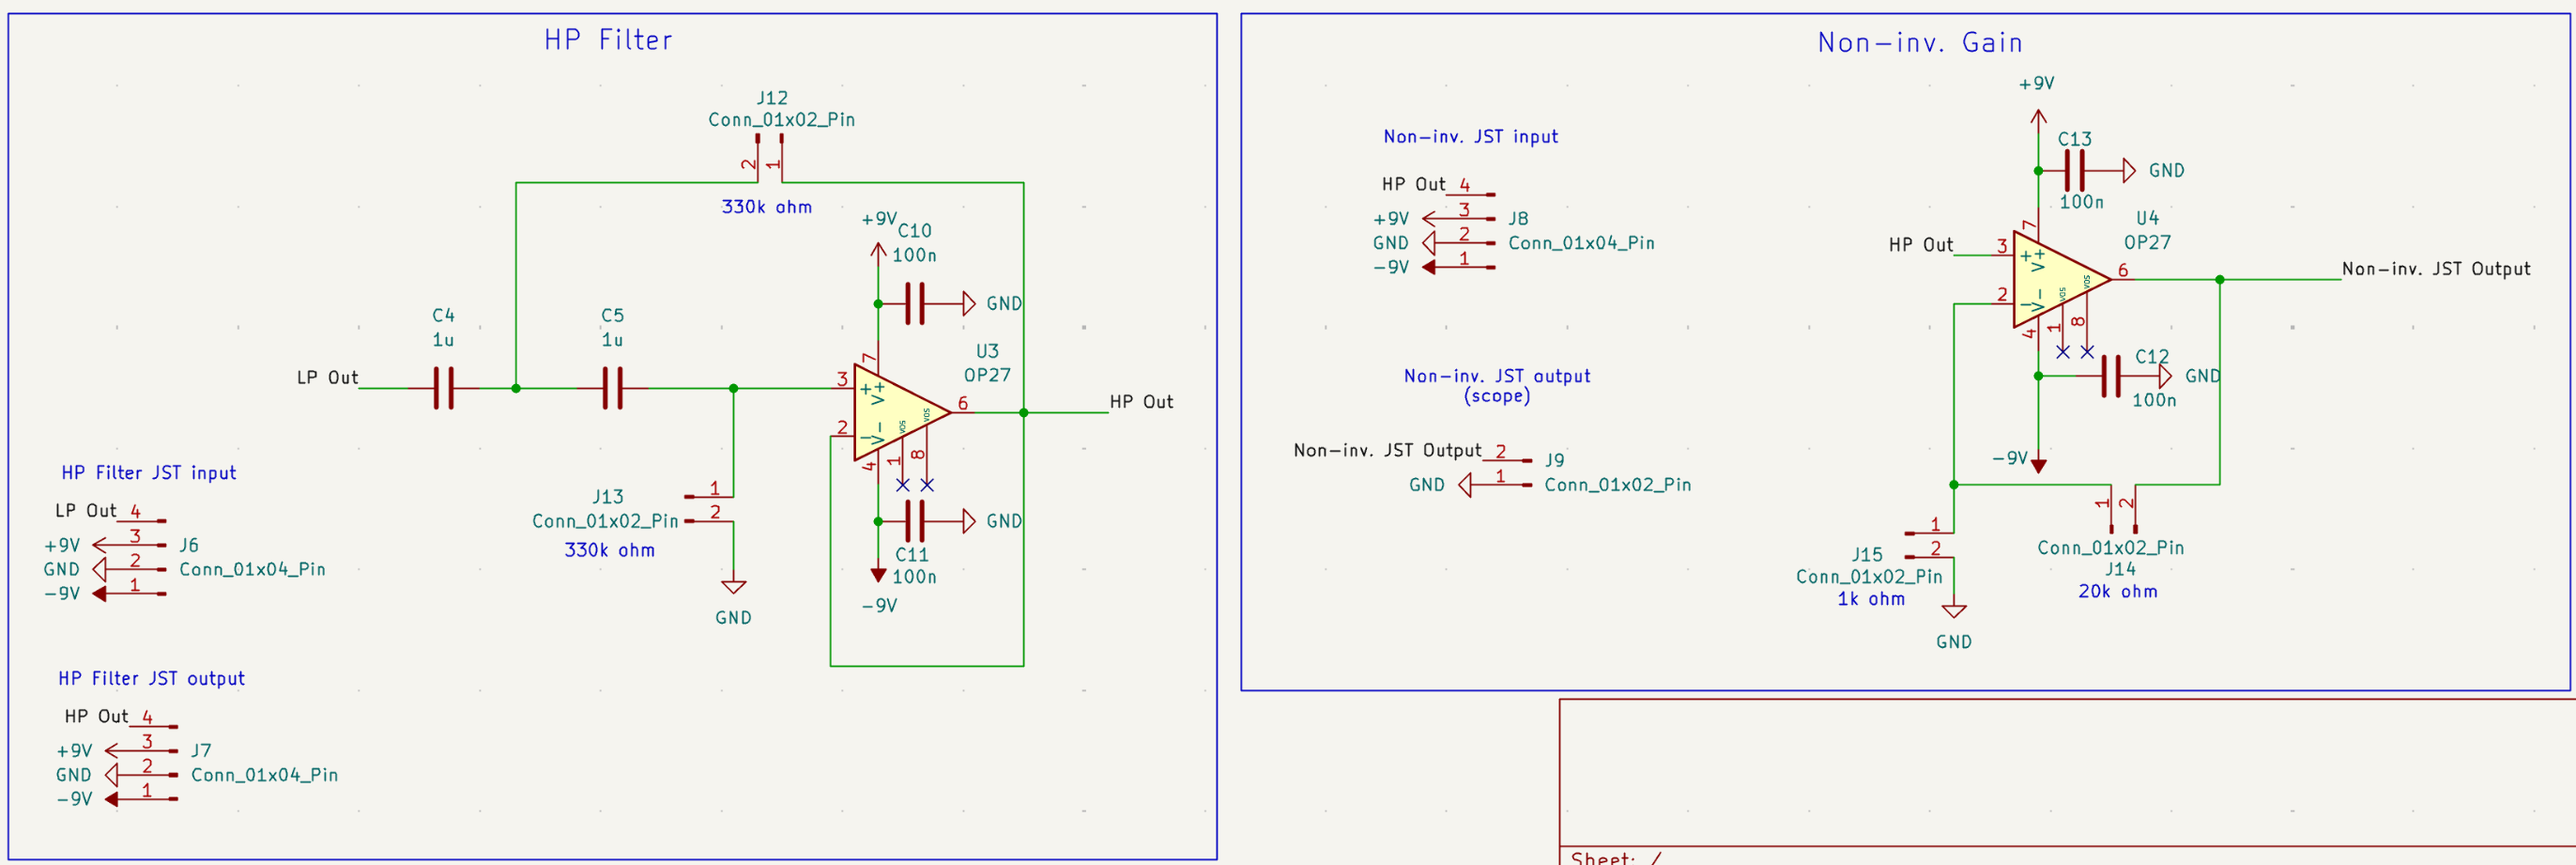
\includegraphics[width=0.8\textwidth]{Pictures/PCB/HIGHPASS_GAIN.png}
         \caption{Skematisk diagram af højpasfilter og den ikke-inverterende forstærker.}
         \label{fig:HP_GAIN}
     \end{subfigure}
     
     \caption{Samlet oversigt over de analoge kredsløbstrin: TIA, filtrering og forstærkning.}
     \label{fig:circuit_stages}
\end{figure}

\begin{figure}[htbp]
    \centering
    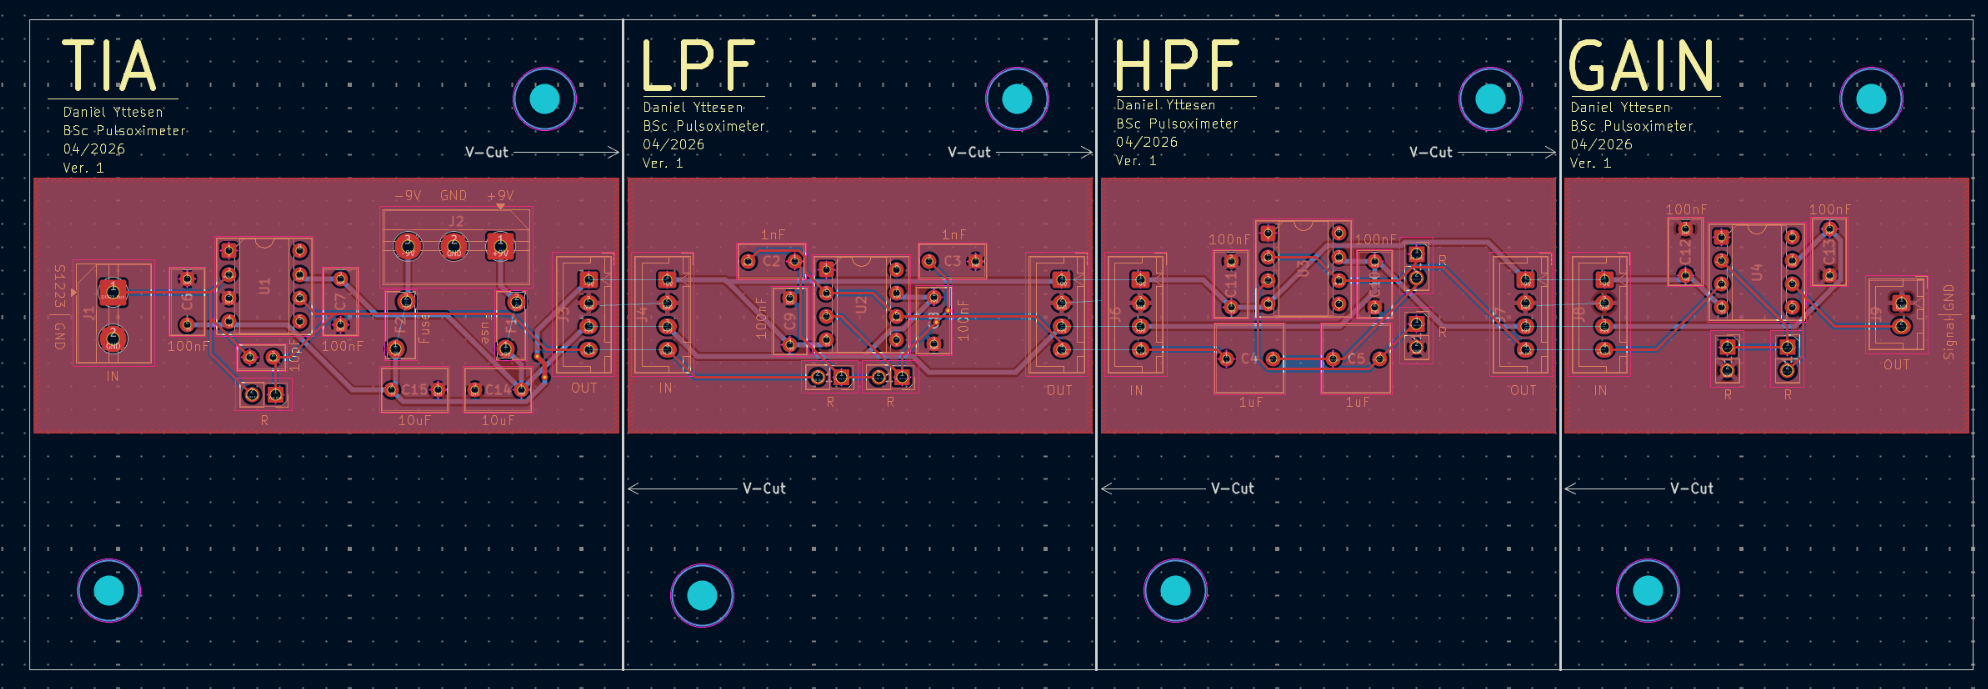
\includegraphics[width=1\textwidth]{Pictures/PCB/PCB.png}
    \caption{Den færdige PCB med traces forbundet.}
    \label{fig:PCB}
\end{figure}

\begin{figure}[htbp]
    \centering
    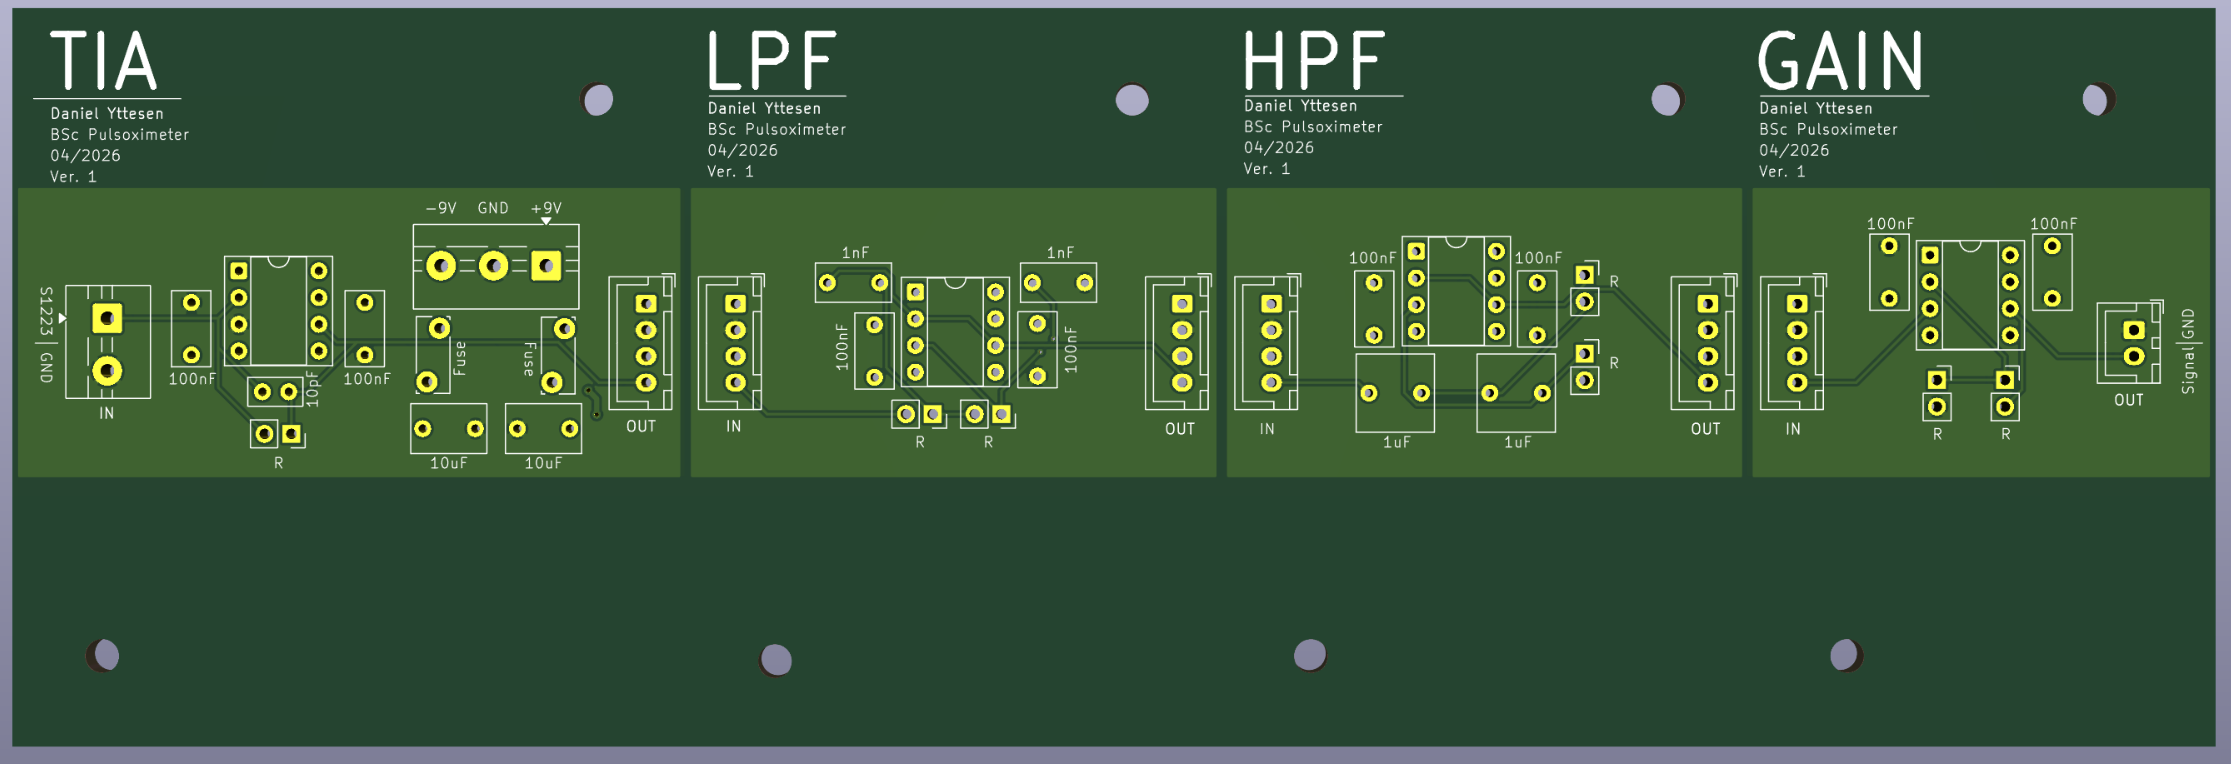
\includegraphics[width=1\textwidth]{Pictures/PCB/PCB3D.png}
    \caption{3D-preview af PCB uden komponenter loddet.}
    \label{fig:PCB_3D}
\end{figure}

\begin{figure}[htbp]
    \centering
    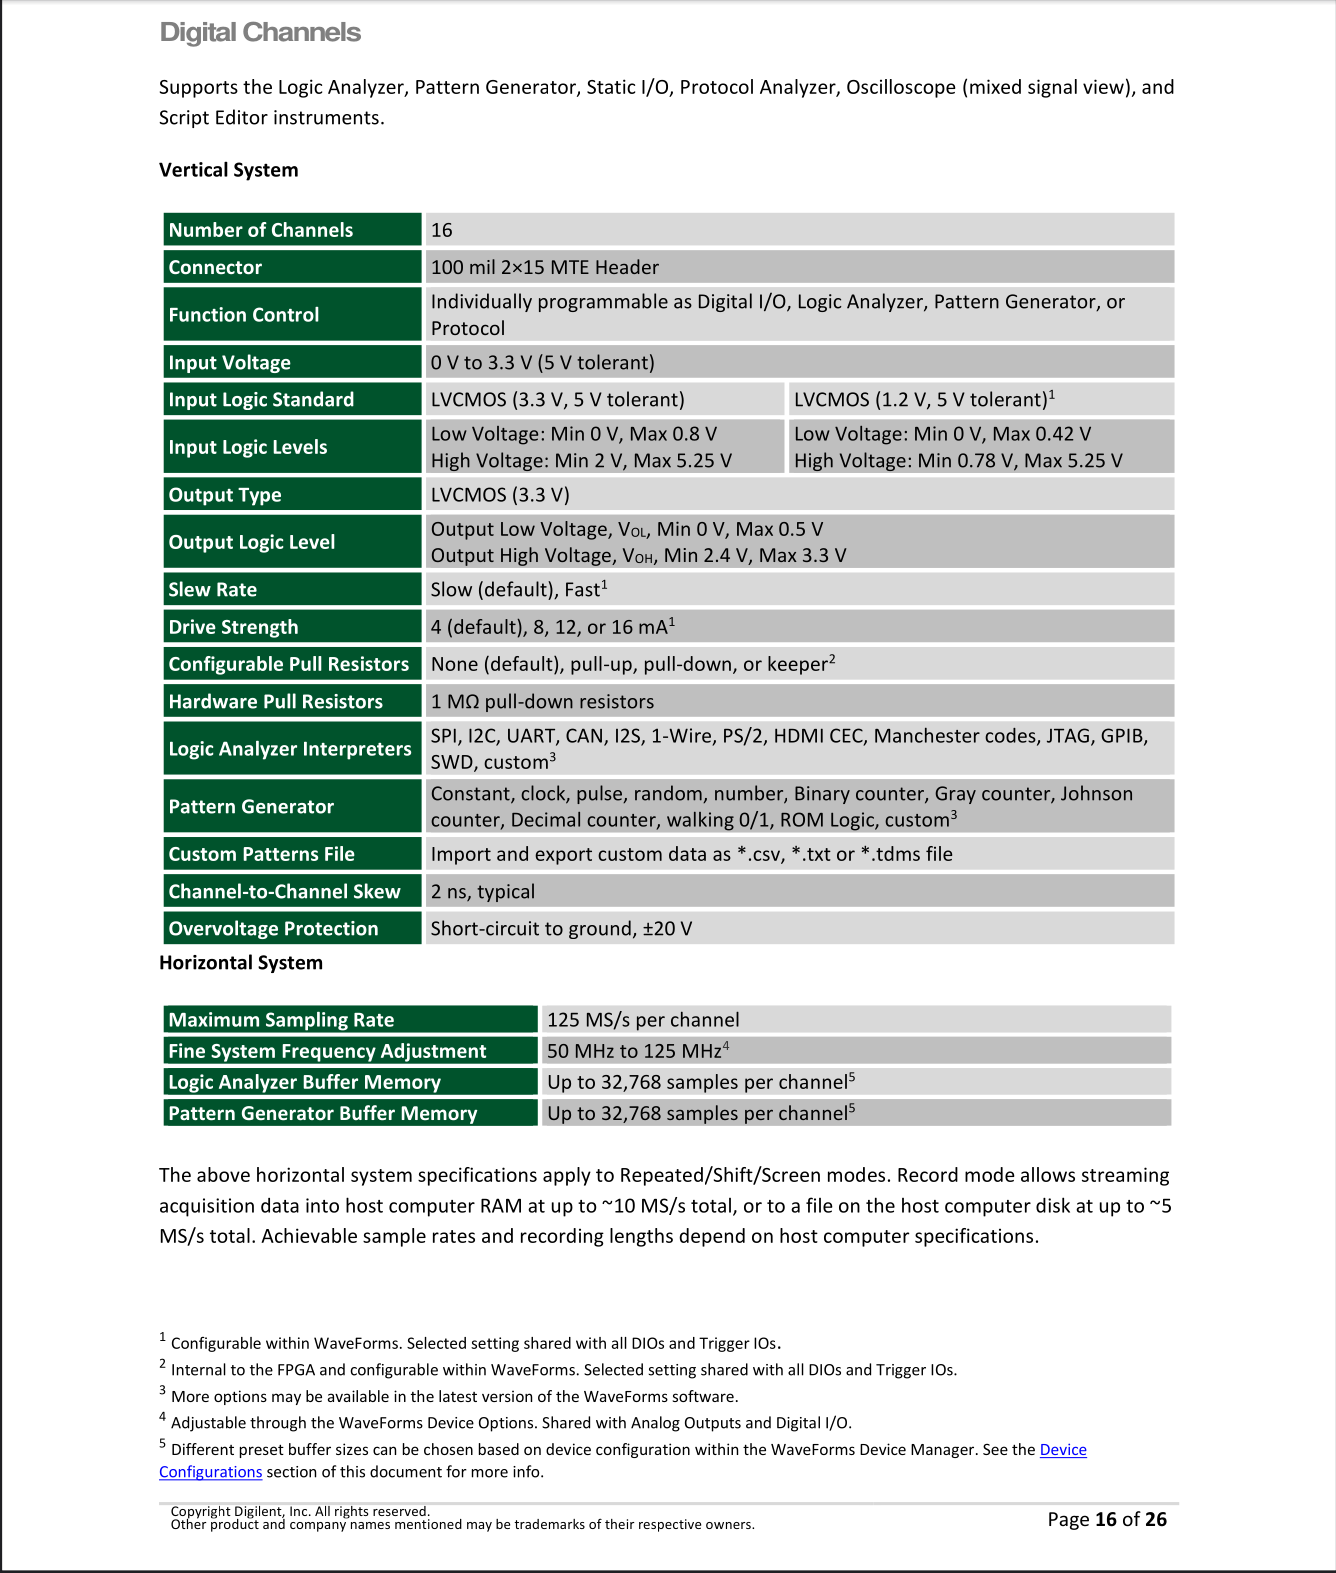
\includegraphics[width=1\textwidth]{Pictures/Datasheets/AD3_Digital.png}
    \caption{Analog Discovery 3 digital output datasheet information.}
    \label{fig:ad3_datasheet}
\end{figure}

\begin{figure}[htbp]
    \centering
    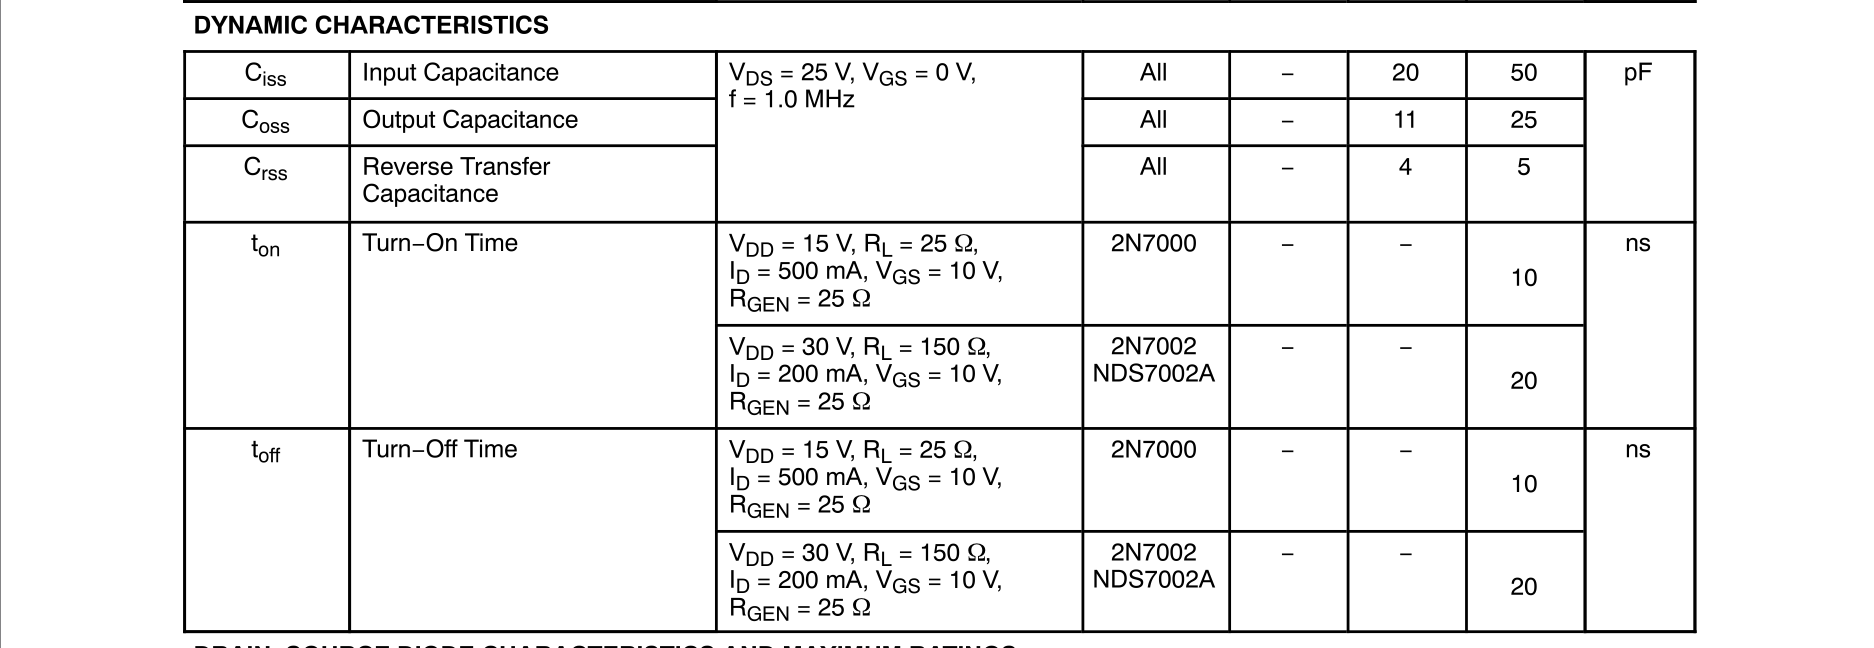
\includegraphics[width=1\textwidth]{Pictures/Datasheets/2N7000_off_on_time.png}
    \caption{2N7000 MOSFET on/off tid fra datasheet fra Mouser.}
    \label{fig:2n7000_datasheet}
\end{figure}

\begin{figure}[htbp]
    \centering
    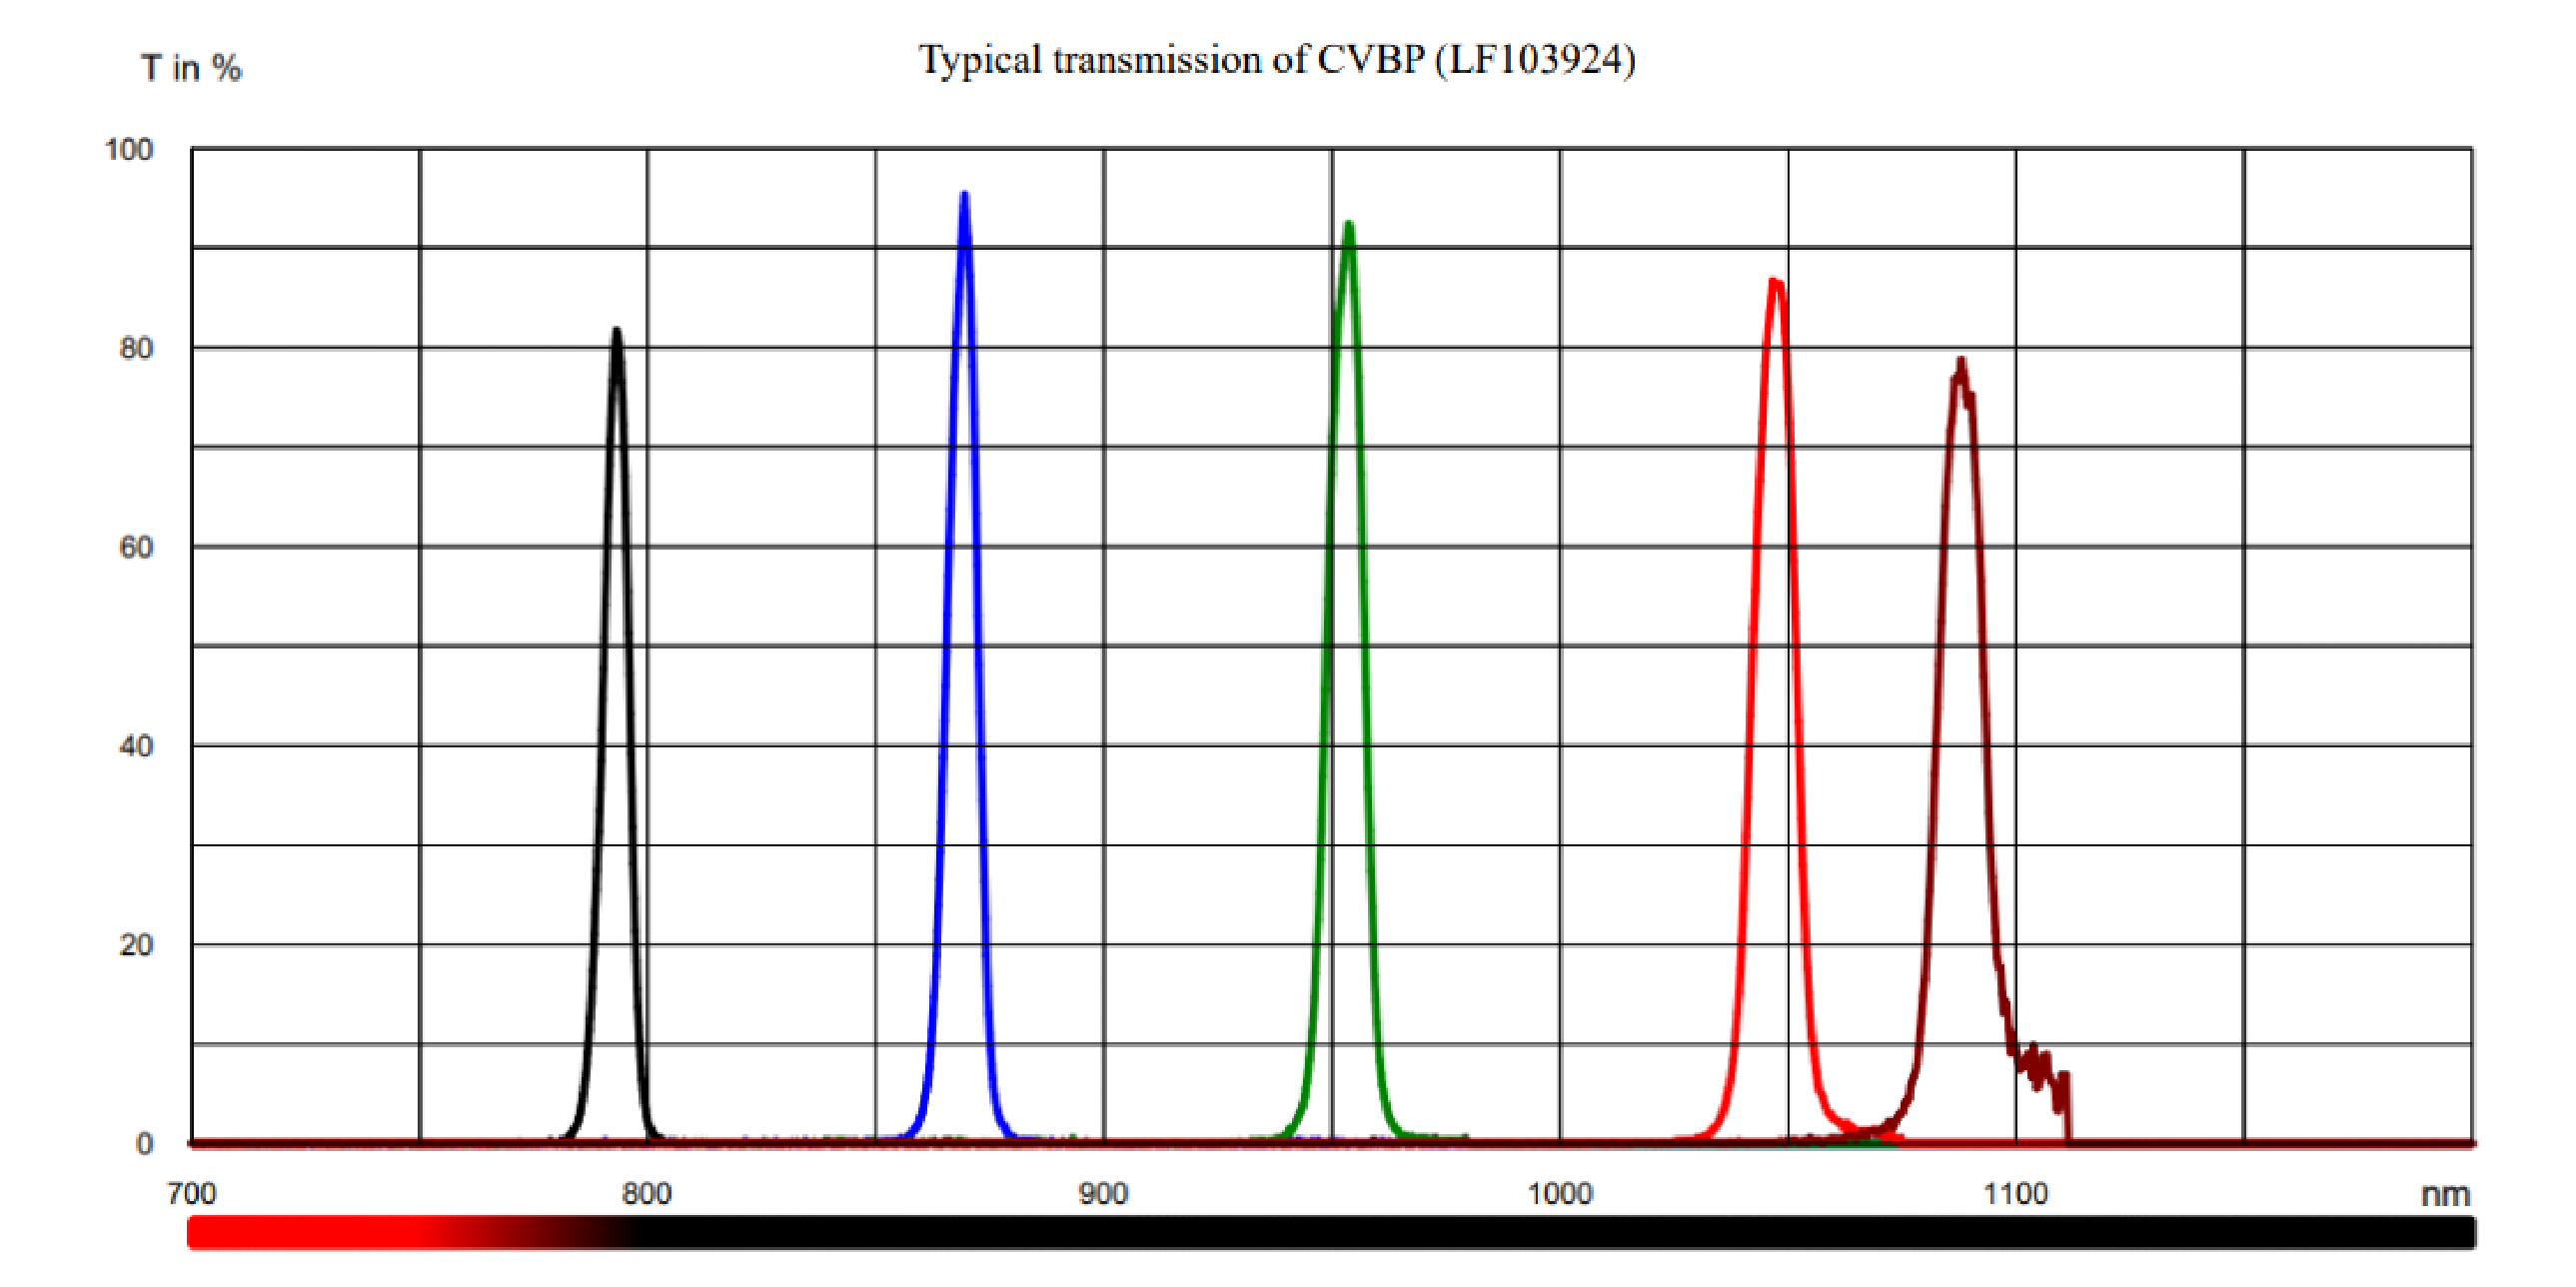
\includegraphics[width=1\textwidth]{Pictures/Datasheets/LVF.png}
    \caption{Relativ transmission i \% for det lineære variable filter (LF103924).}
    \label{fig:LVF}
\end{figure}

\begin{figure}[htbp]
    \centering
    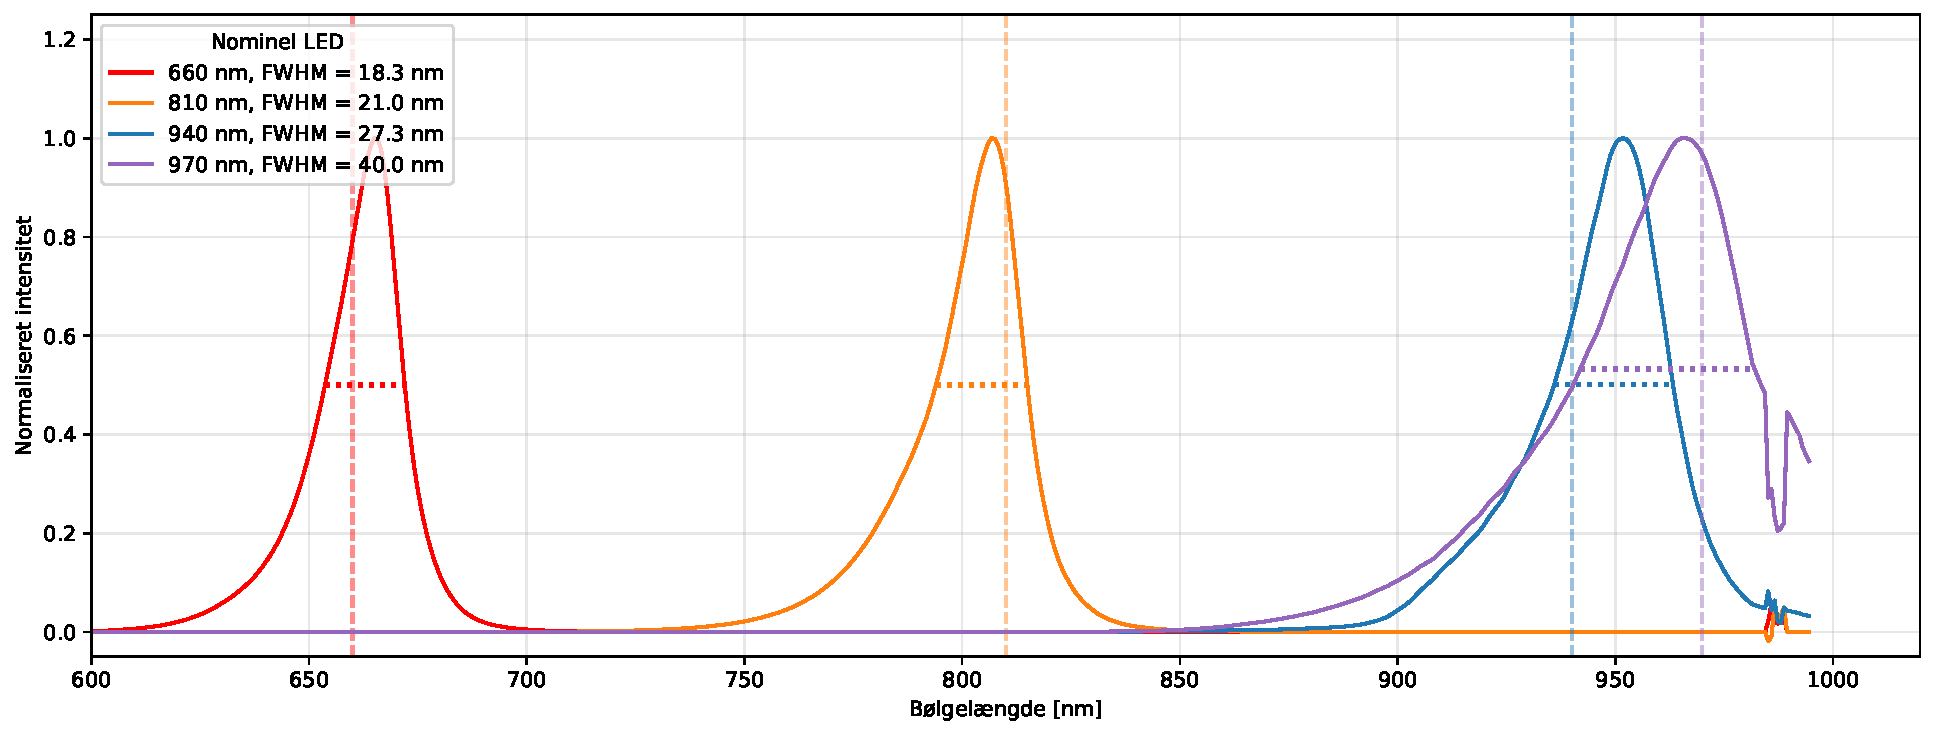
\includegraphics[width=1\textwidth]{Pictures/Graphs/led_spectra_normalized_comparison.pdf}
    \caption{LED spektrum for SMD- og THT-LED'er. Bemærk en "hot" pixel ved ~\SI{970}{nm}, denne skal ignoreres.}
    \label{fig:LED_spektrum}
\end{figure}

\begin{table}[!ht]
    \centering
    \begin{tabular}{|l|l|l|l|l|l|}
    \hline
        LED & Nominel bølgelængde [nm] & Målt peak [nm] & Afvigelse [nm] & FWHM [nm] & Maks intensitet [counts] \\ \hline
        660 nm & 660 & 664.99 & 4.99 & 18.30 & 44.83 \\ \hline
        810 nm & 810 & 806.73 & -3.27 & 20.98 & 43.59 \\ \hline
        940 nm & 940 & 951.79 & 11.79 & 27.25 & 38.79 \\ \hline
        970 nm & 970 & 965.58 & -4.42 & 40.00 & 34.37 \\ \hline
    \end{tabular}
    \caption{Tabel over LED peaks og deres afvigelser.}
    \label{tab:LED_bølgelængder}
\end{table}

\begin{figure}[htbp]
    \centering
    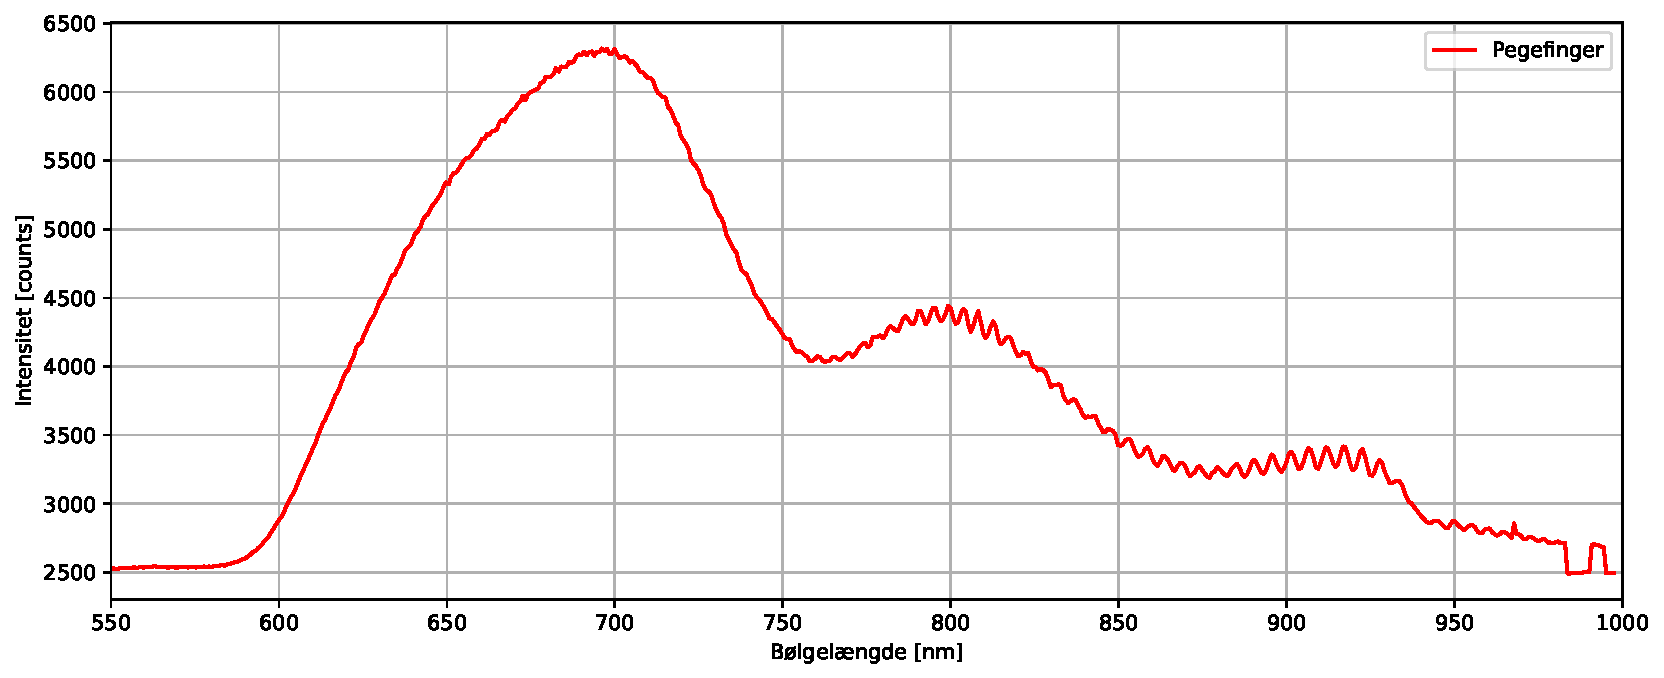
\includegraphics[width=1\textwidth]{Pictures/Graphs/Finger_spektrum.pdf}
    \caption{Spektrum fra gennemlysning af finger med halogenpære.}
    \label{fig:finger_gennemlysning}
\end{figure}

\begin{figure}[htbp]
    \centering
    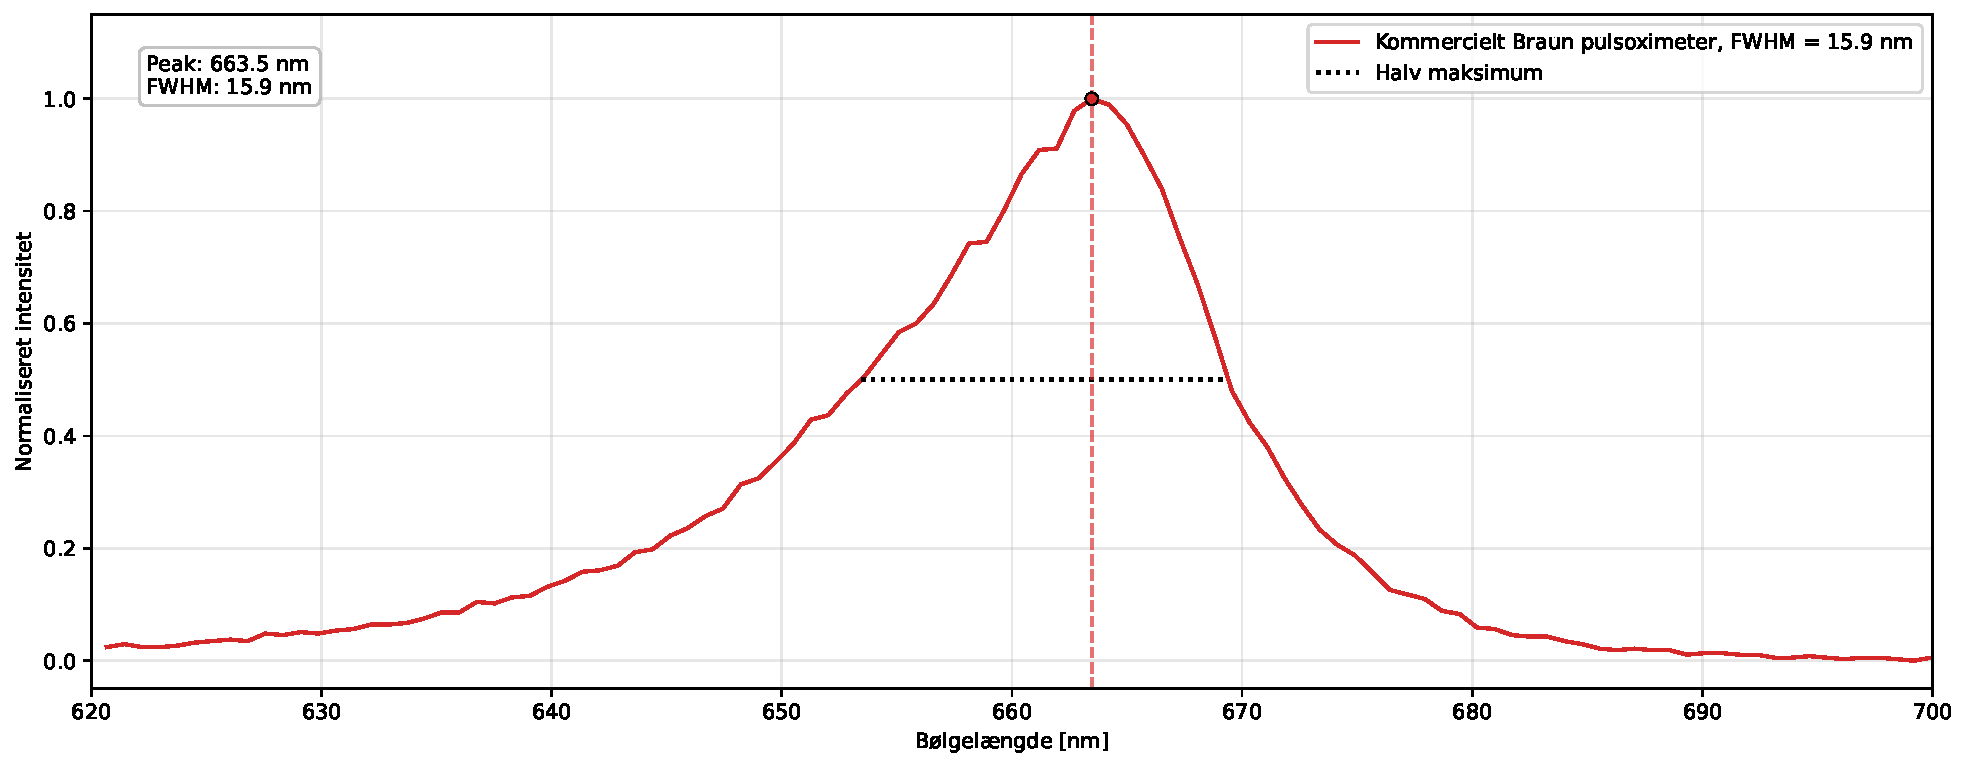
\includegraphics[width=1\textwidth]{Pictures/Graphs/Braun_pulsoximeter.pdf}
    \caption{Spektrum af det kommercielle Braun pulsoximeter}
    \label{fig:Braun_pulsox}
\end{figure}